\section{Cloud Computing}

Internet keeps changing the way people work, learn, communicate and so on. It has influenced from one individual to entire industries. Rapid development of processing and storage technologies helped to reduce the cost of computing while increasing power and availability. This technological advancement provided a realization of a computing model called "Cloud Computing". Users can lease and release the resources like CPU and Storage in an on-demand manner. In general, the cloud computing infrastructure can be divided into two prime roles. One, the infrastructure provider responsible to manage cloud platforms. Second, service-provider, who consume these resources from infrastructure-providers and servers different services to end users. Cloud technologies have influenced the Information Technology (IT) industries and Companies like Google, Microsoft and Amazon provides cloud-platforms which help enterprises to develop, reshape their business models and gain benefits such as No up-front investment in resources since now they can just rent the infrastructure as they uses also known pay-as-you-go pricing model, High scalability, Easy access and important one Risks and maintenance. Using cloud infrastructure means we are simply outsourcing the risks such as hardware failures to the infrastructure providers who are better equipped to manage these risks and decreasing the cost on maintenance and training of staff. In paper \cite{lee2013view}, Author presents results of an economic view of IBM cloud computing engagements \ref{tab:IT_benifits}.


\begin{table}[hb]
    \centering
    \begin{tabular}{|c|c|c|c|}
    \hline
         & Tasks & Traditional Computing &  Cloud Computing \\
    \hline
    \multirow{6}{5em}{Increasing speed and flexibility} & Test provisioning & Weeks & Minutes \\ 
        & Change Management & Months & Days/hours \\ 
        & Release Management & Weeks & Minutes \\
        & Service Access & Administered & Self-service \\ 
        & Standardization & Complex & Reuse/Share \\
        & Metering/billing & Fixed Cost & Variable Cost \\
    \hline
    \multirow{2}{5em}{Reducing Costs} & Server/storage utilization & 10-20\% & 70-90\% \\
        & Payback period & Years & Months \\
    \hline
    \end{tabular}
    \caption{Benifits of Cloud Computing}
    \label{tab:IT_benifits}
\end{table}



\subsection{Overview of cloud Architecture}

The architecture of cloud computing environment is made of sublayers such as Infrastructure as a service (Iaas),  Platform as a Service (Paas) and Software as a Service (SaaS) as show in \Cref{fig:Layers_of_Cloud_Architecture}. Each layer is coupled with layers above or below in a way that each layer can evolved separately allowing applications to be better at management and maintenance. 

\begin{figure}[ht]
    \centering
    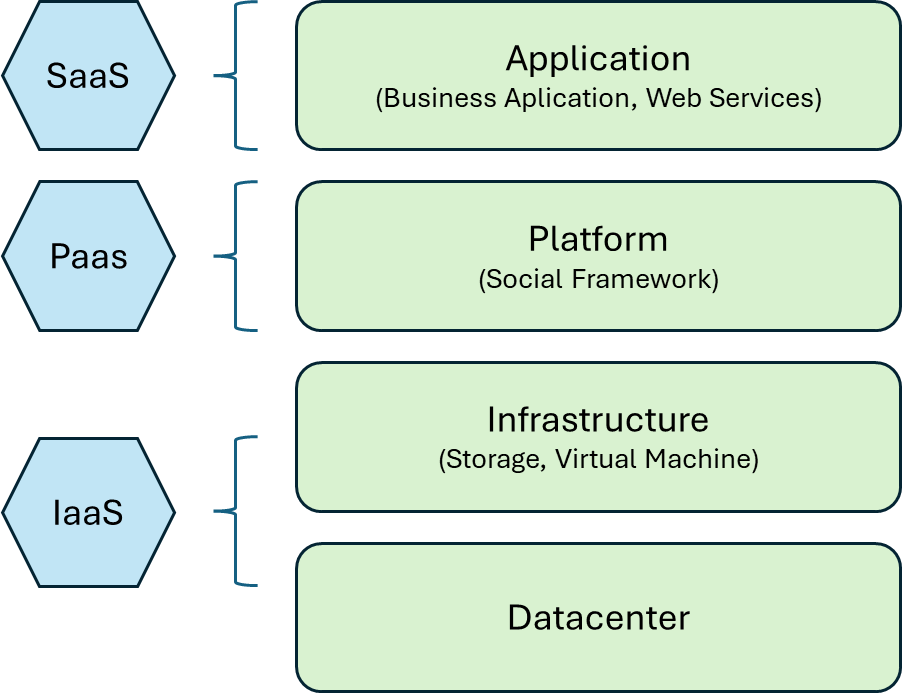
\includegraphics[width=0.5\textwidth]{chapters/images/Cloud_Computing/Cloud_layers.png}
    \caption{Layers of Cloud Architecture}
    \label{fig:Layers_of_Cloud_Architecture}
\end{figure}

\subsubsection{Infrastructure as a Service - IaaS}
The layer IaaS includes resources like data centers that contains servers, routers, power and cooling systems and so on. Therefore, also known as a hardware layer. It also contains the infrastructure layer that includes pool of storage and computing resources like virtualization technologies therefore also known as virtualization layer. IaaS usually refers to providing resources on-demand mostly in forms of Virtual Machines for instance Amazon EC2 \cite{AWS_ec2}. 

\subsubsection{Platform as a Service - PaaS}

This layer is build on top of the infrastructure layer that includes different operating systems and application frameworks. PaaS-provider delivers necessary hardware and software tools over internet for users which allows to focus on deployment and management of their application. 

\subsubsection{Software as a Service - SaaS}

Saas is the layer where the actual cloud application is being served that reaches to end-user and it is at the top of the hierarchy. It is different from ordinary served application in terms of highly-scalable since this layers have automatic-scaling feature to achieve better performance, availability and lower operating cost.

\subsubsection{Machine Learning and Cloud Computing}

Cloud infrastructure outperforms the traditional way of serving the ML models in terms of performance and cost, many of these cloud provider are focusing on developing new architectures that are specifically developed for workloads like neural networks and deep learning, Implementing features like specialized cores to increase matrix operations for instance Google TPUs (Tensor Processing Units) \cite{google_tpu}. In addition, the elasticity, flexibility and economy is making cloud computing more suitable for deploying machine learning models. The different layer model of cloud makes it easy to deploy various infrastructure components on different layers that helps to manage these resources in efficient ways. Cloud providers offers inbuilt PaaS and SaaS a step ahead from low-level offerings like IaaS to enable large-scale computing infrastructures with easy-to-use services in respect to Machine learning "as-a-Service" for end users. Today's data-centers are located in various part of the world. Using services available in PaaS/ SaaS one can deploy their services or product on distributed infrastructures which is accessible trough internet. 

Cloud computing enabled companies to build their products and collaborate on a global level. For instance Hugging face \cite{huggingfacehub} provides a platform where companies or individuals can build their own AI, leverage open source models and technology and make it easy for data scientist, machine learning engineers and developers to collaborate. Users can easily access these models and applications with the hardware capabilities of Google Cloud \cite{Googlecloud} such as TPU instances, Virtual Machines, NVIDIA H100 Tensor Core GPUs \cite{Nvidiagpu} and so on. Currently, there are approx more than 400 thousand models, 150 thousand application and 100 thousand datasets available on hugging face \cite{huggingfacehub}. Some of them may come with copyrights or Licences to use and assets like  Open-Source, anyone can access to these pre-trained models which are already well trained and architected, one can fine-tune it and use it for their downstream tasks with their own datasets or the available datasets without investing on large resource required to set up IT infrastructure to serve high computing services like machine learning on Hugging face by just using internet through their laptops in a pay-as-you-go manner.
